\documentclass{article}
\usepackage{polski}
\usepackage{float}
\usepackage{amsmath}
\usepackage{amssymb}
\usepackage{algorithm}
\makeatletter
\renewcommand{\ALG@name}{Algorytm}
\makeatother
\usepackage{algpseudocode}
\usepackage{graphicx}
\usepackage{geometry}
\graphicspath{ {./plots/} }

\algrenewcommand\algorithmicrequire{\textbf{Dane:}}
\algrenewcommand\algorithmicensure{\textbf{Wynik:}}

\title{Sprawozdanie 4 - Obliczenia Naukowe}
\author{Michał Kallas}
\date{7 grudnia 2024}

\begin{document}

\maketitle

\section{Zadanie 1}
\subsection{Opis problemu}
Napisać funkcję obliczającą ilorazy różnicowe.

\subsection{Opis zagadnienia i rozwiązania}

Ilorazy różnicowe są kluczowym narzędziem w numerycznej analizie funkcji, szczególnie przy konstrukcji interpolacyjnego wielomianu Newtona. Służą do efektywnego obliczania współczynników wielomianu bez potrzeby rozwiązywania układów równań liniowych. 

Dla danych węzłów \(x_0, x_1, \dots, x_n\) oraz odpowiadających im wartości \(f(x_0), f(x_1), \dots, f(x_n)\), ilorazy różnicowe definiujemy rekurencyjnie:
\[
f[x_i] = f(x_i),
\]
\[
f[x_i, x_{i+1}, \dots, x_{i+k}] = \frac{f[x_{i+1}, \dots, x_{i+k}] - f[x_i, \dots, x_{i+k-1}]}{x_{i+k} - x_i}, \quad k \geq 1.
\]

Algorytm polega na stopniowym aktualizowaniu tablicy wartości \(f_x\), która na początku zawiera wartości funkcji \(f(x_i)\).
W procesie aktualizacji obliczamy kolejne ilorazy różnicowe, przechowując je w miejscu wyjściowych wartości.
Złożoność czasowa algorytmu to \( O(n^2) \).

\subsection{Pseudokod}
\begin{algorithm}[H]
\caption{ilorazyRoznicowe}
\begin{algorithmic}[1]
\Require $x$ -- wektor długości $n + 1$ zawierający węzły $x_0, \dots, x_n$, $f$ -- wektor długości $n + 1$ zawierający wartości funkcji w węzłach
\Ensure $f_x$ -- wektor długości $n + 1$ zawierający obliczone ilorazy różnicowe
\State $f_x \gets f$
\For{$i \gets 2$ to $n$}
    \For{$j \gets n$ downto $i$}
        \State $f_x[j] \gets (f_x[j] - f_x[j-1]) / (x[j] - x[j-i+1])$
    \EndFor
\EndFor
\State \Return $f_x$
\end{algorithmic}
\end{algorithm}

\section{Zadanie 2}
\subsection{Opis problemu}
Napisać funkcję obliczającą wartość wielomianu interpolacyjnego stopnia \(n\) w postaci Newtona \(N_n(x)\) w punkcie \(x = t\) za pomocą uogólnionego algorytmu Hornera, w czasie \(O(n)\).

\subsection{Opis zagadnienia i rozwiązania}
Dla danych węzłów \(x_0, x_1, \dots, x_n\) oraz odpowiadających im wartości \(f(x_0), f(x_1), \dots, f(x_n)\), wielomian interpolacyjny Newtona definiujemy jako:

\[
N_n(x) = f[x_0] + f[x_0, x_1](x - x_0) + f[x_0, x_1, x_2](x - x_0)(x - x_1) + \dots + f[x_0, \dots, x_n](x - x_0)(x - x_1)\cdots(x - x_{n-1}),
\]

\noindent Lub, w zwartej formie:

\[
N_n(x) = \sum_{i=0}^n f[x_0, x_1, \dots, x_i] \prod_{j=0}^{i-1} (x - x_j),
\]

gdzie \( f[x_0, x_1, \dots, x_i] \) to i-tego rzędu ilorazy różnicowe, a przy \( i = 0 \) zakładamy, że pusty iloczyn wynosi 1.

Aby obliczyć wartość wielomianu interpolacyjnego w postaci Newtona \( N_n(x) \) w punkcie \( x = t \), wykorzystujemy uogólniony algorytm Hornera.
Algorytm Hornera umożliwia obliczanie wartości takiego wielomianu w sposób efektywny, ze złożonością czasową \( O(n) \).
Zamiast wyliczać poszczególne składniki wielomianu (ilorazy różnicowe i iloczyny $(t - x_i)$) niezależnie i mnożyć je krok po kroku, algorytm Hornera przekształca wzór na $N_n(x)$ w formę umożliwiającą obliczenia w sposób ,,odwrócony''.

Rozpoczynamy od współczynnika $f[x_0, x_1, \dots, x_n]$, który odpowiada najwyższemu stopniowi wielomianu, i rekurencyjnie obliczamy wartość wielomianu, dodając kolejne składniki od końca.
W każdej iteracji wynik obliczeń z poprzedniego kroku jest mnożony przez $(t - x_i)$, a następnie dodawany jest kolejny współczynnik.

\subsection{Pseudokod}
\begin{algorithm}[H]
\caption{warNewton}
\begin{algorithmic}[1]
\Require $x$ -- wektor długości $n + 1$ zawierający węzły $x_0, \dots, x_n$, $f_x$ -- wektor długości $n + 1$ zawierający ilorazy różnicowe, $t$ -- punkt, w którym należy obliczyć wartość wielomianu
\Ensure $nt$ -- wartość wielomianu w punkcie $t$
\State $nt \gets f_x[n]$
\For{$i \gets n-1$ downto $1$}
    \State $nt \gets nt \cdot (t - x[i]) + f_x[i]$
\EndFor
\State \Return $nt$
\end{algorithmic}
\end{algorithm}

\section{Zadanie 3}
\subsection{Opis problemu}
Znając współczynniki wielomianu interpolacyjnego w postaci Newtona
\[
c_0 = f[x_0], \quad c_1 = f[x_0, x_1], \quad c_2 = f[x_0, x_1, x_2], \quad \dots, \quad c_n = f[x_0, \dots, x_n] \quad (\text{ilorazy różnicowe})
\]
oraz węzły \(x_0, x_1, \dots, x_n\), napisać funkcję obliczającą, w czasie \(O(n^2)\), współczynniki jego postaci naturalnej
\[
a_n x^n + a_{n-1} x^{n-1} + \dots + a_1 x + a_0.
\]

\subsection{Opis zagadnienia i rozwiązania}
Wielomian interpolacyjny w postaci Newtona można przekształcić do postaci naturalnej, czyli:
\[
P(x) = a_n x^n + a_{n-1} x^{n-1} + \dots + a_1 x + a_0 = \sum_{i=0}^n a_i x^i.
\]
Bardzo istotną obserwacją jest to, że współczynnik $c_n = f_x[n]$ z postaci Newtona jest równy współczynnikowi $a_n$ przy najwyższej potędze w postaci naturalnej.
Kolejne współczynniki możemy wyliczać na podstawie poprzednich oraz wartości ilorazów różnicowych i węzłów, przy okazji aktualizując współczynniki przy wyższych potęgach poprzez odjęcie aktualnego węzła.
Algorytm działa ze złożonością czasową \( O(n^2) \).

Dla pierwszych 3 iteracji wyniki wyglądają następująco:
$$a_n = c_n$$
$$a_{n-1} = c_{n-1} + c_n \cdot \sum_{i=0}^{n-1}-x_i$$
$$a_{n-2} = c_{n-2} + c_{n-1} \cdot \sum_{i=0}^{n-2}-x_i + c_{n} \cdot \sum_{i=j=0, i<j}^{n-1}(-x_i) (-x_j)$$

\subsection{Pseudokod}
\begin{algorithm}[H]
\caption{naturalna}
\begin{algorithmic}[1]
\Require $x$ -- wektor długości $n + 1$ zawierający węzły $x_0, \dots, x_n$, $f_x$ -- wektor długości $n + 1$ zawierający ilorazy różnicowe
\Ensure $a$ -- wektor długości $n + 1$ zawierający obliczone współczynniki postaci naturalnej
\State $a \gets \text{wektor zer o rozmiarze } n$
\State $a[n] \gets f_x[n]$
\For{$i \gets n-1$ downto $1$}
    \State $a[i] \gets f_x[i] - x[i] \cdot a[i+1]$
    \For{$j \gets i+1$ to $n-1$}
        \State $a[j] \gets a[j] - x[i] \cdot a[j+1]$
    \EndFor
\EndFor
\State \Return $a$
\end{algorithmic}
\end{algorithm}

\section{Zadanie 4}
\subsection{Opis problemu}
Napisać funkcję \texttt{rysujNnfx}, która zinterpoluje zadaną funkcję $f(x)$ w przedziale $[a, b]$ za pomocą wielomianu interpolacyjnego stopnia $n$ w postaci Newtona.
Następnie narysuje wielomian interpolacyjny i interpolowaną funkcję

\subsection{Rozwiązanie}
W funkcji \texttt{rysujNnfx} na początku wyznaczyłem węzły interpolacyjne \( x_k \), które są równomiernie rozmieszczone w przedziale \( [a, b] \) z określoną odległością \( h = \frac{b - a}{n} \).
Węzły są obliczane w następujący sposób:
\[
x_k = a + k \cdot h \quad \text{dla} \quad k = 0, 1, \dots, n.
\]
Po obliczeniu węzłów, obliczyłem wartości funkcji w tych punktach(\( f(x_k) \)).
Wartości te zostały następnie użyte do wyznaczenia ilorazów różnicowych za pomocą funkcji \texttt{ilorazyRoznicowe}.

Kolejnym krokiem było obliczenie wartości wielomianu interpolacyjnego oraz funkcji \( f \) w punktach, które zostały zadane do rysowania wykresu.
Dla \( x_i \), gdzie \( x_i \) to punkty w przedziale \( [a, b] \), obliczane są wartości wielomianu interpolacyjnego za pomocą funkcji \texttt{warNewton}, a także \( f(x_i) \).
W celu otrzymania dokładniejszego wykresu, obliczam te wartości dla \( 100 n \) punktów w przedziale \( [a, b] \).

Po wyliczeniu wartości wielomianu interpolacyjnego oraz funkcji \( f \), rysowany jest wykres.

\section{Zadanie 5}
\subsection{Opis problemu}
Przetestować funkcję \texttt{rysujNnfx(f,a,b,n)} na następujących przykładach:
\begin{itemize}
    \item (a) $f_1(x) = e^x$, $[0, 1]$, $n = 5, 10, 15$,
    \item (b) $f_2(x) = x^2 \sin x$, $[-1, 1]$, $n = 5, 10, 15$.
\end{itemize}

\subsection{Wykresy}
\begin{figure}[H]
\centering
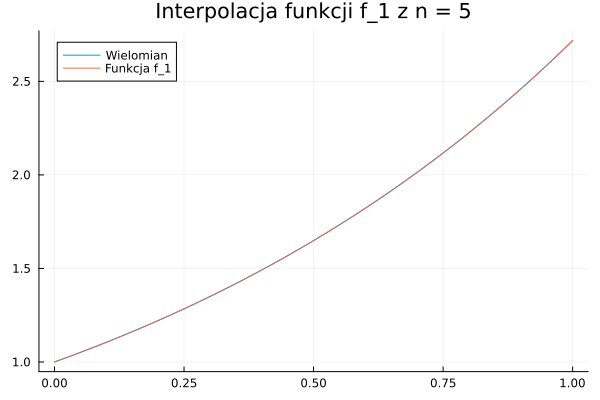
\includegraphics[width=0.75\textwidth]{task5_f1_n5.png}
\caption{Wykres uzyskany przez funkcję \texttt{rysujNnfx($e^x$, 0, 1, 5)}.}
\end{figure}

\begin{figure}[H]
\centering
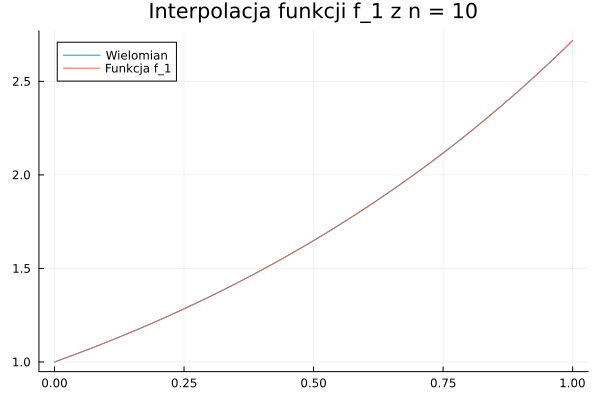
\includegraphics[width=0.75\textwidth]{task5_f1_n10.png}
\caption{Wykres uzyskany przez funkcję \texttt{rysujNnfx($e^x$, 0, 1, 10)}.}
\end{figure}

\begin{figure}[H]
\centering
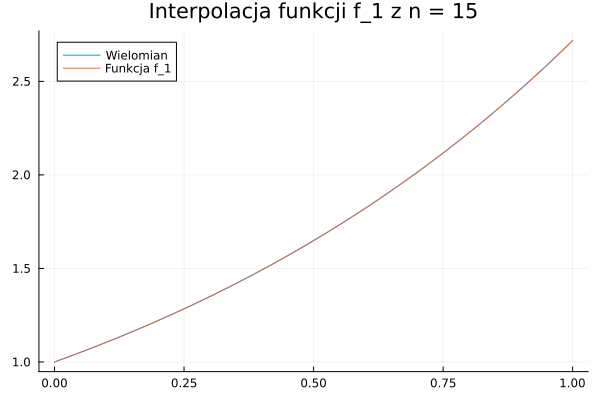
\includegraphics[width=0.75\textwidth]{task5_f1_n15.png}
\caption{Wykres uzyskany przez funkcję \texttt{rysujNnfx($e^x$, 0, 1, 15)}.}
\end{figure}

\begin{figure}[H]
\centering
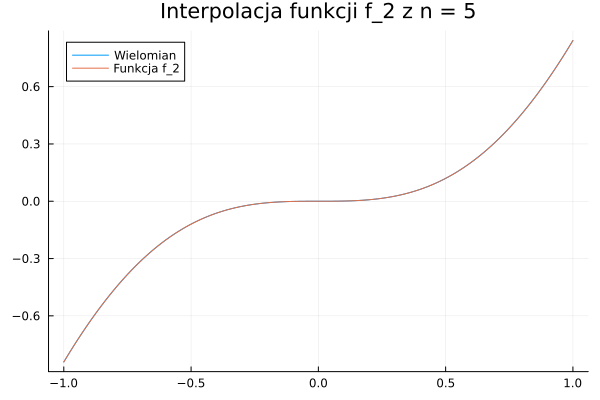
\includegraphics[width=0.75\textwidth]{task5_f2_n5.png}
\caption{Wykres uzyskany przez funkcję \texttt{rysujNnfx($x^2 \sin x$, -1, 1, 5)}.}
\end{figure}

\begin{figure}[H]
\centering
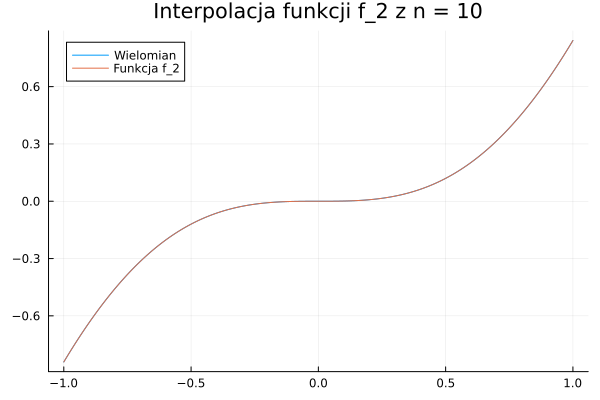
\includegraphics[width=0.75\textwidth]{task5_f2_n10.png}
\caption{Wykres uzyskany przez funkcję \texttt{rysujNnfx($x^2 \sin x$, -1, 1, 10)}.}
\end{figure}

\begin{figure}[H]
\centering
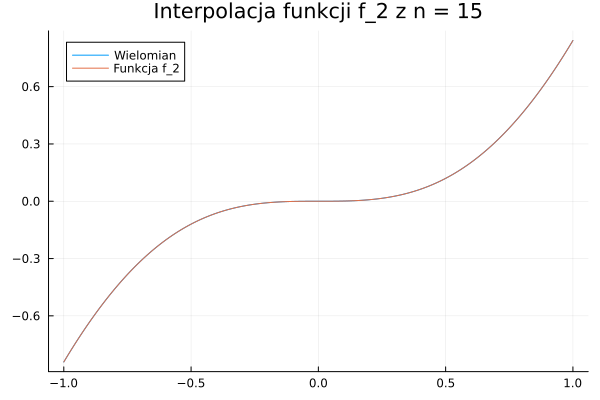
\includegraphics[width=0.75\textwidth]{task5_f2_n15.png}
\caption{Wykres uzyskany przez funkcję \texttt{rysujNnfx($x^2 \sin x$, -1, 1, 15)}.}
\end{figure}

\subsection{Obserwacje i wnioski}
Jak widać na wykresach, zarówno dla $f_1$, jak i $f_2$ interpolacja działa bardzo dobrze.
Wartości wielomianów interpolacyjnch wszystkich sprawdzanych stopni pokrywają się z wartościami funkcji na całych przedziałach.


\section{Zadanie 6}
\subsection{Opis problemu}
Przetestować funkcję \texttt{rysujNnfx(f,a,b,n)} na następujących przykładach (zjawisko rozbieżności):
\begin{itemize}
    \item (a) $f_1(x) = |x|$, $[-1, 1]$, $n = 5, 10, 15$,
    \item (b) $f_2(x) = \frac{1}{1+x^2}$, $[-5, 5]$, $n = 5, 10, 15$ (zjawisko Runge'go).
\end{itemize}

\subsection{Wykresy}
\begin{figure}[H]
\centering
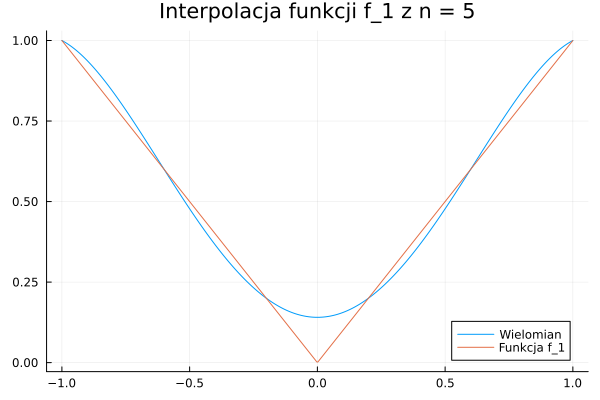
\includegraphics[width=0.75\textwidth]{task6_f1_n5.png}
\caption{Wykres uzyskany przez funkcję \texttt{rysujNnfx($|x|$, -1, 1, 5)}.}
\end{figure}

\begin{figure}[H]
\centering
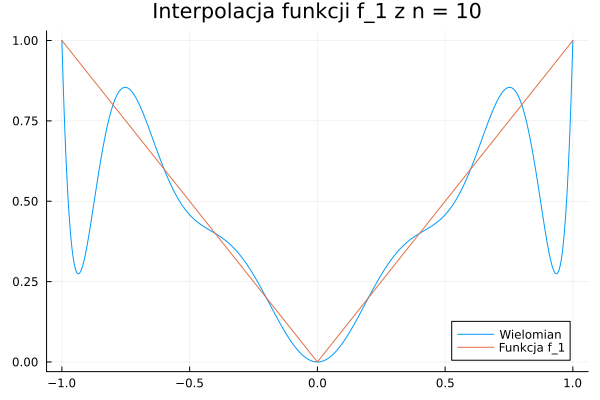
\includegraphics[width=0.75\textwidth]{task6_f1_n10.png}
\caption{Wykres uzyskany przez funkcję \texttt{rysujNnfx($|x|$, -1, 1, 10)}.}
\end{figure}

\begin{figure}[H]
\centering
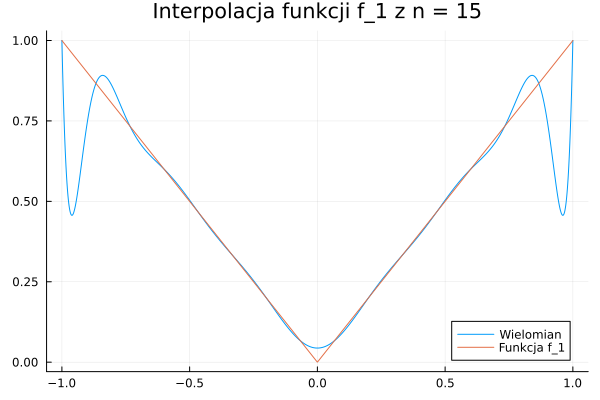
\includegraphics[width=0.75\textwidth]{task6_f1_n15.png}
\caption{Wykres uzyskany przez funkcję \texttt{rysujNnfx($|x|$, -1, 1, 15)}.}
\end{figure}

\begin{figure}[H]
\centering
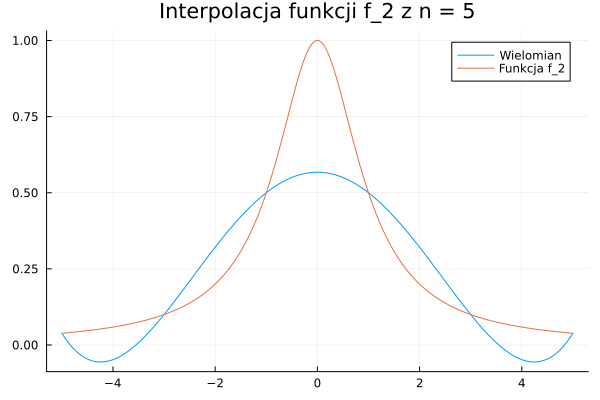
\includegraphics[width=0.75\textwidth]{task6_f2_n5.png}
\caption{Wykres uzyskany przez funkcję \texttt{rysujNnfx($\frac{1}{1+x^2}$, -5, 5, 5)}.}
\end{figure}

\begin{figure}[H]
\centering
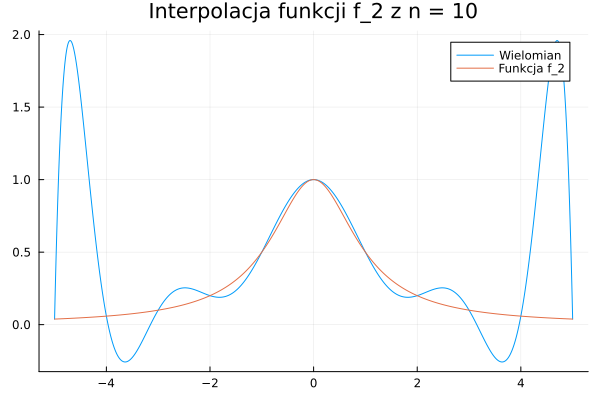
\includegraphics[width=0.75\textwidth]{task6_f2_n10.png}
\caption{Wykres uzyskany przez funkcję \texttt{rysujNnfx($\frac{1}{1+x^2}$, -5, 5, 10)}.}
\end{figure}

\begin{figure}[H]
\centering
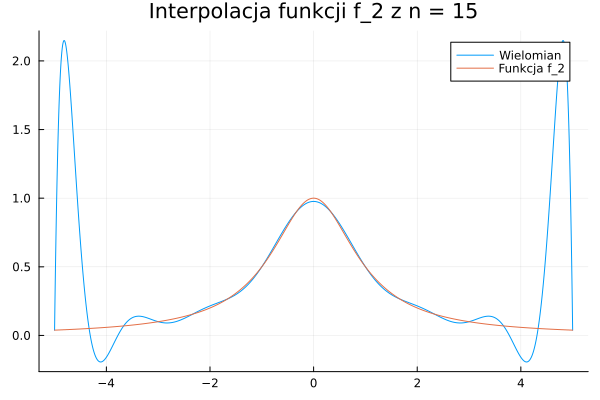
\includegraphics[width=0.75\textwidth]{task6_f2_n15.png}
\caption{Wykres uzyskany przez funkcję \texttt{rysujNnfx($\frac{1}{1+x^2}$, -5, 5, 15)}.}
\end{figure}

\subsection{Obserwacje i wnioski}
W tym przypadku, zarówno dla $f_1$, jak i $f_2$ interpolacja nie zadziałała tak dobrze.
Zauważalne są różnice pomiędzy wartościami funkcji, a wielomianu interpolowanego.

Przy zwiększeniu stopnia wielomianu dokładność interpolacji maleje, co jest szczególnie widoczne na krańcach przedziału.
Jest to całkiem nieoczywiste zjawisko, jako że dostajemy gorsze wyniki, mimo większej ilości węzłów.
Intuicyjnie, większy stopień powinien prowadzić do lepszego przybliżenia.

Taką sytuację określa się mianem zjawiskia Runge'go.
Błąd wielomianu interpolacyjnego wyliczonego za pomocą równoodległych węzłów staje się coraz większy wraz ze wzrostem jego stopnia.

Dobrym rozwiązaniem tego problemu są węzły Czebyszewa.
Dzięki nim, występuje więcej węzłów w miejscach, które są trudne do przybliżenia, co zwiększa jego dokładność.

\end{document}
